%\section{Variations of Hamiltonian parameters across quantum critical point}
%\label{rtripcqt}

\section{Protocol}

 In the following, we focus on the round-trip protocol between gapped phase in the Kitaev
wire described by the Hamiltonian \eqref{Hkitaev} with antiperiodic boundary condition
($\hat c_{L+1} = - \hat c_1$). To fix the notation, we will take:
\be{notation}
	w = \mu - \mu_c \pt
\ee

We investigate the critical dynamics of closed systems assuming quasi-adiabatic variation
of the parameter $w$ across the critical point $w_c = 0$, e.g. following the standard KZ
procedure:

\begin{itemize}
\item[$\bullet$] One starts from the ground state of the many-body system at
	$w_i < 0$, given by $\ket{\Psi(t=t_i)} \equiv \ket{\Psi_0(w_i)}$.
  
\item[$\bullet$] Then the out-equilibrium unitary dynamics, ruled by the
	Schr\"odinger equation
	\begin{equation}
		{{\rm d} \, \ket{\Psi(t)} \over {\rm d} t} =
		- i \, \hat H[w(t)] \, \ket{\Psi(t)} \,,
	\label{unitdyn}
	\end{equation}
	arises from a linear dependence of the time-dependent parameter $w(t)$, such as
	\begin{equation}
		w(t) = t/t_s \,,
		\label{wtkz}
	\end{equation}
	up to a final value $w_f>0$. Therefore the KZ protocol starts at time 
	$t_i = t_s \, w_i<0$ and stops at $t_f= t_s \, w_f>0$.  The
	parameter $t_s$ denotes the time scale of the slow variations of the
	Hamiltonian parameter $w$.

\item[$\bullet$]
	Then, for $t>t_f$, we complete the cycle by descreasing $w$ from $w_f$ to the
	original value $w_i$ with the same time scale $t_s$.

\end{itemize}

To reduce the number of the free parameter, we consider a symmetric round-trip protocol
with:
\ba{symmKZ}
	w_\star &= w_f = -w_i \cm \\
	t_\star &= t_f = -t_i \pt
\ea

The resulting out-of-equilibrium evolution of the system can be
investigated by monitoring observables and correlations at fixed time.
One may consider the evolution of the adiabaticity function:
\ba{adiab}
	A(t) = \abs*{  \braket{\Psi_0[h(t)] | \Psi(t)}} \cm
%  \approx 
%  1 - |\langle \, \Psi_0[h(t)] \, | \, \Psi(t) \, \rangle|\,,
\ea
where $\ket{\Psi_0[w(t)]}$ is the ground state of the
Hamiltonian $\hat H[w(t)]$, i.e. at instantaneous values of $w(t)$,
while $\ket{\Psi(t)}$ is the actual time-dependent state
evolving according to the Schr\"odinger equation (\ref{unitdyn}).  The
adiabaticity function measures the overlap of the time-dependent state
with the corresponding ground state of the Hamiltonian at the same
$w(t)$. Since the protocol starts from the ground state associated
with $w_i=w(t_i)$, we trivially have $A(t_i) = 1$.  If the quantum
evolution is adiabatic, then $A(t)=1$ at any time.  In the general
case arising from the above KZ protocol, $A(t)$ is expected to depart
from the initial value due to the impossibility of the system to
adiabatically follow the changes of the function $w(t)$ across its
critical value $w=0$.

Note however that this is strictly true in the infinite-volume limit.  In system of
finite size $L$, there is always a sufficiently large time scale $t_s$, so that the system 
can evolve adiabatically, essentially because finite-size systems are always gapped, 
although the gap $\Delta$ at the CQT gets suppressed as $\Delta \sim L^{-z}$. The
interplay between the size $L$ and the time scale $t_s$ gives rise to nontrivial 
out-of-equilibrium scaling behaviors, which can be studied within finite-size scaling (FSS)
frameworks~\cite{rossini2020dynamic, rossini2021coherent}.\\

Another interessant quantities useful to monitor the out-of equilibrium dynamics are:
\begin{itemize}
	\item
		the substract definition of the particle density:
		\ba{partden}
			\rho_s(t) = \braket{\Psi(t) | c_x^\dagger c_x | \Psi(t)}
			- \rho_c \pc
		\ea
		where $\rho_c$ is its corrispondent value at the critical point in the 
		infinite-volume limit.
	\item
		The fermionic correlation functions:
		\ba{corrC}
			C(x,t) =\braket{\Psi(t)| c_j^\dagger c_{j+x} + {\rm h.c.}| 
			\Psi(t)} \cm
		\ea
		with $i,j \in [1,L/2]$ considering the translation invariance due to ABC.
\end{itemize}


\section{Dynamic Finite Size Scaling}

Let us discuss the scaling whitin a dynamic RG framework. In the limit of slow variation
of the driven parameter $w$, the dynamic scaling is dependent from the universality class
while we cross the CQT point. In this situation, the critical divergent of the equilibrium
relaxation time $t_r$ is correlated with the scale time $t_s$ of the variation of the
driven parameter $w$. 
In particular, $t_r$ behaves as: 
\be{trelax}
	t_r \sim \xi^{z} \sim \abs{w}^{-z\nu} \pt
\ee

In this way, the interplay of the various dimensionful scales of the problem (such as the 
time $t$, the time scale $t_s$, the system size $L$ and the energy gap 
$\Delta \sim L^{-z}$) characterizes the flux of the RG transformations, leading to the 
scaling laws for observables constructed from a local operator $O({\bm x})$.
The dynamic FSS of its expectation value $O_s$ and its two-point correlation
function $G_O$ are expected to obey homogeneous scaling laws~\cite{rossini2021coherent}:
\ba{dynamicfsskz}
	O^{(a/b)}_s(t,t_s,w_\star,L) &\simeq  b^{-y_o} {\cal O}
				(b^{-z}t, b^{y_w}w(t), b^{y_w}w_\star,b^{-1}L) \cm \\
	G^{(a/b)}_O(\bm x, t, t_s, w_\star, L) &\simeq  b^{-2y_o} {\cal G}
			(b^{-1}\bm x,b^{-z}t, b^{y_w}w(t), b^{y_w}w_\star,b^{-1}L) \pc
\ea
where $b$ is an arbitrary lenght scale and the superscripts $(a)$ and $(b)$ indicate the
outward and return trajectories.

By fixing $b = L$, we find the dynamic FSS of the KZ procedure. Then, the asympotic
dynamic behavior is obtained by taking $t_s \to \infty$ and $L \to \infty$, while the
following scaling are kept fixed:
\ba{scalingKZ}
	K = w(t)L^{y_w} \cm &\qquad \Upsilon = t_s/L^{\zeta}\cm \\
	\Theta_\star = w_\star t_s^{1-\kappa} \cm &\qquad \Theta 
				= w(t)t_s^{1-\kappa} = t/t_s^\kappa \cm
\ea
(note that $K = \Upsilon^{\kappa-1}\Theta$) where:
\ba{expscalingKZ}
	\zeta = y_w + z \cm \quad \kappa = z/\zeta \cm \quad 1-\kappa = y_w/\zeta \pt
\ea
The previous scaling variable and the corresponding exponent derive from the application
of the relations $b=L$ and $w(t)=t/t_s$ to the scaling laws Eqs.\eqref{dynamicfsskz}.\\

The corresponding dynamic scaling laws of the adiabaticity \eqref{adiab} and the 
correlation functions \eqref{corrC} are given by:
\ba{scalobsKZ}
	A^{(a/b)}(t,t_s,w_\star,L) &\simeq 
		{\cal A}^{(a/b)}(\Upsilon,\Theta,\Theta_\star) \cm \\
	\label{scalobsKZ1}
	C^{(a,b)}(x,t,t_s,w_\star,L) &\simeq L^{-2y_c} 
		{\cal C}^{(a/b)}(x/L,\Upsilon,\Theta,\Theta_\star) \pc
\ea
where $y_c$ is the RG dimension associated with the operator $\hat c$ and equal to $1/2$
\cite{S99}. Note that the values of these observables after the full cycle are different
from those at the beginning:
\be{disa-b}
	{\cal A}^{(b)} (\Upsilon, \Theta=-\Theta_\star, \Theta_\star) \neq
	{\cal A}^{(a)} (\Upsilon, \Theta=-\Theta_\star, \Theta_\star) \cm
\ee
they coincide only in the adiabatic limit, i.e. $\Upsilon \to \infty$, when the 
time-evolved system explores all the equilibrium state at the corresponding value of 
$\Theta(t)$.

In the above scaling behavior \eqref{scalobsKZ}-\eqref{scalobsKZ1}, the scaling parameter
$\Theta$ plays a fundamental role. While in the classic hysteresis-like scenario the 
relaxational dynamic lead to a well-defined dynamic scaling when keeping $w_\star > 0$
\cite{tarantelli2022out} fixed, the quantum case is more problematic. The radid 
oscillations, due to the unitary dynamics, make the return somehow chaotic and extremely
sensitive to the protocol parameters. This implies, also, a non-convergent value at the
end of the round-trip protocol in the large-$\Theta_\star$ limit.

The dynamic scaling is realized only when keeping $\Theta_\star$ fixed, in fact the 
relative quantum phase behave consistently with the scaling laws.
 
\section{Numerical Results}

\begin{figure}[!t]
	\centering
	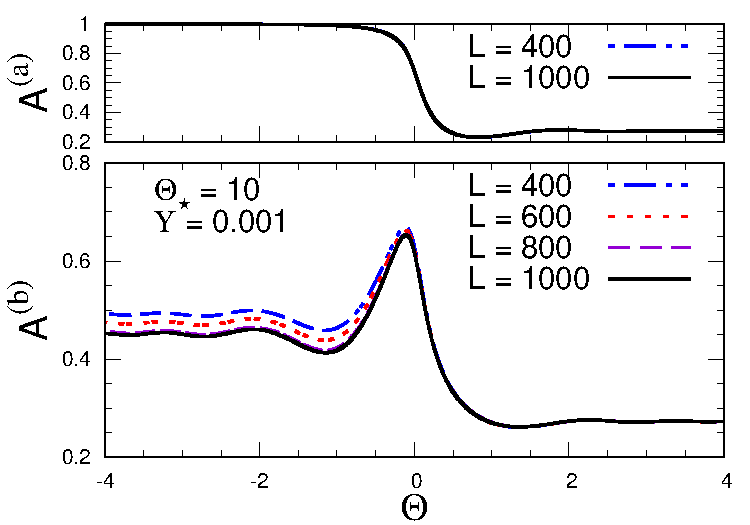
\includegraphics[width=10cm]{imm/headKITY0001Th10A.pdf}
	\caption{Round-trip dynamic FSS within the quantum Kitaev
	taev wire for a finite $\Theta_\star = 10$. We show results for the adiabaticity
	function $A(t, t_s , w_\star, L)$ at fixed $\Upsilon =t_s /L^\zeta = 0.001$
	and $\Theta_\star = w_\star L^{1-\kappa} = 10$, for the outward (top) and return 
	(bottom) branches of the round-trip KZ protocol, versus
	$\Theta = w(t)L^{1-\kappa}$ , for various size $L$ up to $L = 1000$. The values
	of the exponents $y_w$ , $\zeta$, and $\kappa$ are reported in 
	Eq.\eqref{criticalexpKZ}. The numerical results clearly support the 
	dynamic scaling behavior given in Eq. \eqref{scalobsKZ}.}
	\label{akitaevfss}
\end{figure}


The numerical results are computed using a Kitaev wire with exact diagonalization
techniques based on Nambu operators~\cite{bla86}. The resolution of the time-dependent
Schr\"odinger equation is obtained through the $4^{\rm th}$ order Runge-Kutta method.

This approach allows us to present simulation for lattice size $L$ up to $L=1000$. It is
sufficient to achieve a robust evidence of the dynamic FSS outlined in the previous 
section. The corresponding critical exponents, associated with the quantum Kitaev model
with driving chemical potential, are:
\be{criticalexpKZ}
	y_w = 1 \cm \qquad \zeta = 2 \cm \qquad \kappa = 1/2 \pt
\ee

We show numerical results for round-trip KZ protocols keeping $\Theta_\star$ finite, see
Figs. \ref{akitaevfss} and \ref{ckitaevfss}, for the adiabaticity and the correlation
functions. These plots support the dynamic FSS reported in the scaling laws in Eqs.
\eqref{scalobsKZ}-\eqref{scalobsKZ1}.

\begin{figure}[!t]
        \centering
        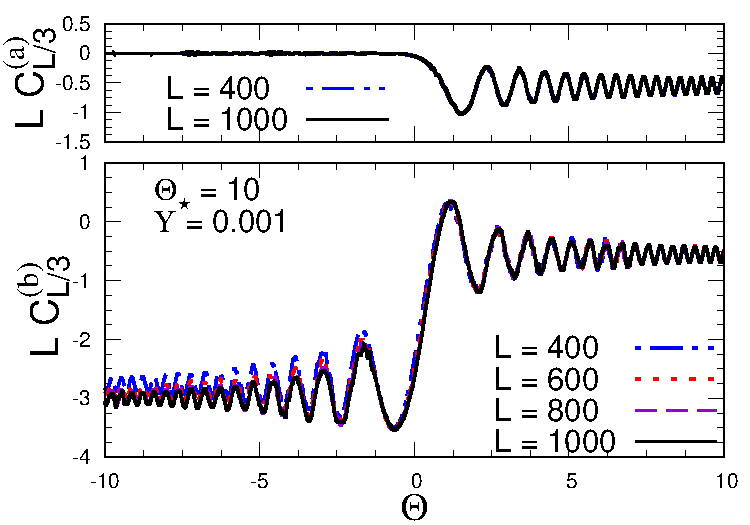
\includegraphics[width=10cm]{imm/headKITY0001Th10C.pdf}
        \caption{Round-trip dynamic FSS within the quantum Kitaev
        taev wire for a finite $\Theta_\star$. We show results for two-point
        function $C(x,t, t_s , w_\star, L)$ at fixed 
	$X = x/L = 1/3 \,, \,\,\Upsilon =t_s /L^\zeta = 0.001$
        and $\Theta_\star = w_\star L^{1-\kappa} = 10$, for the outward (top) and return
        (bottom) branches of the round-trip KZ protocol, versus
        $\Theta = w(t)L^{1-\kappa}$ , for various size $L$ up to $L = 1000$.
	The numerical results clearly support the
        dynamic scaling behavior given in Eq. \eqref{scalobsKZ1}.}
	\label{ckitaevfss}
\end{figure}


\subsection{The large-$\Theta_\star$ limit}

We now discuss the large-$\Theta_\star$ limit which turns out to be quite problematic
in quantum round-trip KZ protocols. To observe it, we focus on the end of the outward
branch $(a)$ and of the return branch (b) for KZ protocols with different $\Theta_\star$
(the "inversion-point"), to check their large-$\Theta_\star$ convergence, for some 
interval of values of $\Theta_\star$ and fixed $L$.\\

The observables at the end
of the outward branch oscillate, with a frequency that becomes larger and larger with 
increasing $\Theta_\star$, as shown in Fig. \ref{oscill} , and the
oscillations observed after the whole cycle are strongly
correlated to those at the end of the first branch, doubling the frequency.

The above results strongly suggest that in quantum many-body systems the 
large-$\Theta_\star$ limit of the dynamic KZ scaling does not exist along the return 
trajectories, and, as a consequence, no dynamic scaling is observed along the
return trip when $w_\star$ is kept fixed and finite in the
round-trip KZ protocols.\\

However, we stress that the dynamic scaling behavior
is nicely observed when keeping $\Theta_\star$ fixed, even along the
return trajectory. This may be related to fact that, when
keeping $\Theta_\star$ fixed, the time scaling variable $\Theta_\star$ remains 
finite, therefore the time variable is always rescaled 
consistently with the time scale of the equilibrium quantum
transition, provided by the inverse gap at the transition,
i.e. $\Delta \sim  L^{-z}$ at the critical point, or $\Delta \sim \lambda^{-z}$ 
in the thermodynamic limit, where $\lambda$ is the KZ length scale %\cite{45}
. As a consequence, the interval of values of $w(t)$ remains 
limited within a small interval around the transition, which
becomes smaller and smaller in the large-size limit, as
$\abs{w} \lesssim L^{-y_w}$ , and the relative quantum phases behave
consistently with the scaling laws.

\begin{figure}[!t]
        \centering
        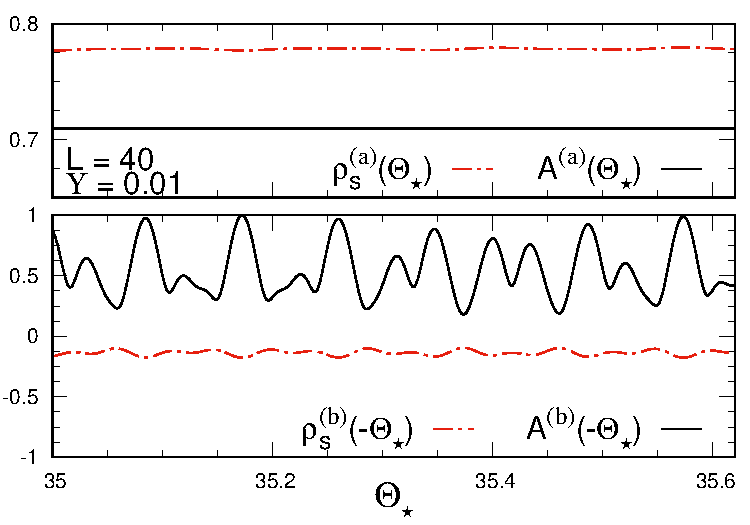
\includegraphics[width=7cm]{imm/diffThstaru001T35l40.pdf}
	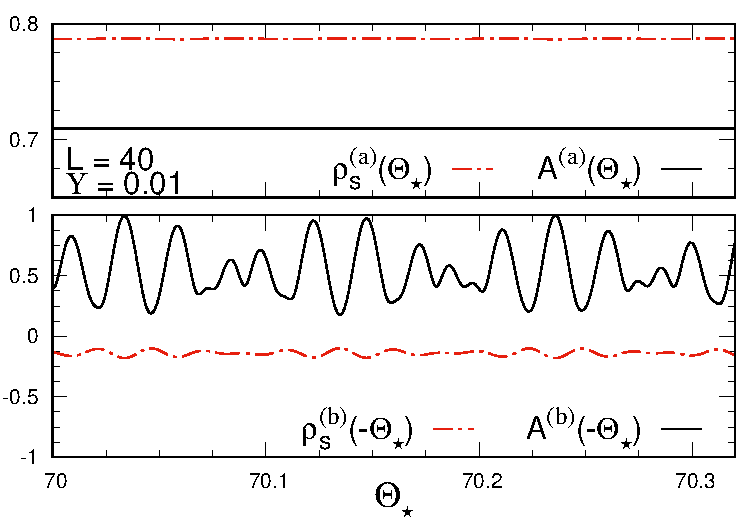
\includegraphics[width=7cm]{imm/diffThstaru001T70l40.pdf}
	\caption{Behavior of the subtracted particle density $\rho_s$
	 and the adiabaticity function $A$ for the Kitaev wire,
	for fixed $L = 40\,,\,\, \Upsilon = 0.01$ versus $\Theta_\star$ , 
	close to $\Theta_\star = 70$
	(bottom figure) and $\Theta_\star = 35$ (top figure). In each figure,
	the top plot the values of $\rho_s^{(a)}$ and $A^{(a)}$ at the end of the
	outward branch, corresponding to $\Theta = \Theta_\star$ , while the bottom
	plot shows the values of $\rho_s^{(b)}$ and $A^{(b)}$ at the end of the return
	branch, corresponding to $\Theta = -\Theta_\star$. Again, the comparison
	of the top and bottom figures show that the oscillations tend
	to become more frequent with increasing $\Theta_\star$. }
	\label{oscill}
\end{figure}


\section{Summary}

We address these issues within many-body model
undergoing quantum transitions, exploiting a
unified RG framework, where general dynamic scaling
laws are derived in the large-$t_s$ and large-$L$ limits. In particular,
we extend the RG framework already developed for standard KZ protocols.


The observation of 
scaling behavior along the return way turns out to be more
problematic, due to the persistence of rapidly 
oscillating relative phases between the relevant quantum states.
They make the return way extremely sensitive to the 
parameters of the protocol, such as the extreme value $w_f$
and the size $L$ of the system. This is essentially related
to the quantum nature of the dynamics. Indeed there are
some notable similarities with the behavior of quantum
two-level models subject to round-trip protocols, 
analogous the well-known Landau-Zener-Stückelberg problem~\cite{tarantelli2022out}.\\

\begin{comment}
The same results are also observed in the case of the quantum Ising model with the
driving of the longitudinal magnetization field~\cite{tarantelli2022out}. 
Note that, in the case of one-dimensional quantum Ising model, the slow variation of the
longitudinal field across the CQT point brings the system from a gapped condition to another
gapped condition, i.e. move the system from disorder to disorder through a CQT. Therefore,
this is not the standard situation of the KZ problem related to the defect production going 
from the disorder to the order phases.

The corresponding 
results generalized all the above discussion on the Kitaev model. In fact, using the 
Jordan-Wigner transformation we can interpret the driving protocol of the chemical potential
in the Kitaev wire as the driving of the transverse magnetization field in the transverse
quantum Ising model (neglecting the boundary conditions since the thermodynamic limit are
independent from them at the critical point).\\

Analogous issues are investigated at first-order, where dynamic scaling behaviors emerge 
as well, see details \cite{tarantelli2023out}.

\end{comment}

